
\week{Things That Follow Rules}

Rules are all around us. Some rules are set by nature. Others are made by people.

When you throw a ball into the air, you know it's going to come down. This is a simple example of a
natural rule.

\hint{You don't need to read the margins, unless you're extra curious!}

% TODO: figure of ball going up and down

Rules can sound boring, but certain rules can be very interesting, as we'll see later on.

This chapter is about simple rules that cause interesting behavior --
without anyone thinking, planning, or deciding.

Even things that seem random run on rules. For example, if you let the
air out of a filled balloon, the balloon will whiz around the
room.\curious{Even systems that look random often follow perfectly
  strict rules. When a system is sensitive to tiny details, we call it
  \term{chaotic}. This can make prediction hard, even if the rules are
  simple}
Where it lands might seem random, but if you knew the rules
of physics \emph{and} every tiny detail of the room, you could
figure out what would happen to the balloon before you let it
go.
\didyouknow{All of known physics can be described by just \emph{nine}
  rules \parencite{motionmountain}!}
You don't need to believe this yet -- the important idea is that surprising behavior can still came from strict rules.

You may be wondering what this has to do with computers. The answer
is: \textbf{any system that follows rules is a kind of computer.}

\begin{BigIdeaBox}
A \term{computer} is just a system that follows rules!
\end{BigIdeaBox}

\section{Building a Computer}

\huh{Wait! Is everything a computer?}{In nature,
  we discover rules. In computers, we design them. However, some
  scientists really do think of the universe as a kind of
  computer. Others disagree. But it doesn't really matter, because all
  rule-following systems can be studied in the same way. This branch
  of science is called \term{computer science}.}
When we build a computer, we have to think about the sorts of things
we want to compute. An extremely simple example of a computer is a lamp. This follows two very simple rules:

\begin{enumerate}[label={\textcolor{IdeaBlue}{\sffamily \textbf{Rule \arabic*}}}, leftmargin=4em]
\item When you flip the switch on, the light goes on.
\item When you flip the switch off, the light goes off.
\end{enumerate}

The lamp follows rules, but its rules are pretty simple.

Usually, we only call something a computer if it does more interesting
things. To make computers like that, we have to set up the rules
carefully.  \curious{A lamp follows rules, but it cannot store
  information or combine rules in new ways. What separates simple
  machines from powerful computers is not just the number of rules,
  but how rules combine.}

\subsection{Turing Tumble}

The \emph{Turing Tumble} game lets you set up a system that follows
simple rules. The game has two colors of marbles: \textcolor{marbleblue}{blue} on the left and
\textcolor{marblered}{red} on the right. The marbles fall down and hit different pieces along
the way.\huh{Why are we using marbles in a computer programming class?}{Marbles move slowly enough that we can see the rules happening. Inside a real computer, the same ideas happen billions of times a second. That would be too hard to see!}

Each piece follows a simple rule. Some pieces always send marbles the
same direction. Other pieces can change what they do depending on what
happened before. When a marble reaches the bottom, it can hit a lever
that releases a new marble of a certain color.\didyouknow{It may seem
  crazy, but this is \emph{exactly} how real computers are
  built. Instead of marbles, engineers use even smaller balls called
  electrons.}

The marbles accumulate at the very end, and this shows us the order in
which the marbles were released. For example, consider the computer in
\prettyref{fig:bluemarble}. What happens when a blue marble is released?

Let's walk through it. You start by releasing a blue marble from the left marble bank. The marble
makes its way down until it hits the blue lever. Upon hitting the blue lever, \emph{another} blue
marble is released. No red marble is ever released. As the game progresses, the board accumulates blue marbles in its
bottom bank. We call this bank its \term{output}.

By changing how the pieces are laid out, you can make interesting computers that arrange marbles in
different ways.
\didyouknow{
  You can play Turing Tumble on a computer at the website \href{https://jessecrossen.github.io/ttsim}{https://jessecrossen.github.io/ttsim}\\
  \begin{center}
    \qrcode{https://jessecrossen.github.io/ttsim}
  \end{center}
}

\begin{figure}[ht]
  \fixfigure
  \centering

\begin{tikzpicture}
  \begin{ttboard}[label={Turing Tumble}, blue marbles = 8, red marbles = 8, blue marbles released = 1, output=\ttpieces{bbb}]

  % Place a Bit at (col=3,row=6) with state 0
    %    \TTBit[state=0, /tt/piece/name=topbit]{3}{0}
    \TTRamp[left, /tt/piece/name=topbit]{3}{0}
    \TTRampRun{2}{1}{\TTRows - 2}
%    \TTRamp[right]{4}{1}
%    \TTRamp[right]{5}{2}
%    \TTRamp[right]{6}{3}
%    \TTRampRun{6}{4}{\TTRows - 2}

    \draw[<-, color=IdeaBlue, opacity=0.8, line width=0.2cm] ($(leftentrance) + ({-0.1*\TTXUnit},{-0.5*\TTYUnit})$) to [bend left] (-0.5, 6) node [text width=2.5cm, anchor=east, color=black] {\footnotesize \sffamily As each blue marble is released,
      this piece forces it towards the right. The next piece forces it left, all the way down until it hits the blue lever.};
    \draw[<-,color=IdeaBlue, opacity=0.8, line width=0.2cm] ($(leftleverweight) + ({-0.1*\TTXUnit},{0.5*\TTYUnit})$) to[bend right] (-0.5, 2) node[text width=2.5cm, anchor=east, color=black] {\footnotesize \sffamily When the lever here is hit, another \emph{blue} marble is released};
    \draw[<-,color=IdeaBlue, opacity=0.8, line width=0.2cm] ($(\TTBoardRight, \TTBoardBottom) + ({-0.5 * \TTXUnit}, {0.2*\TTYUnit})$) to [bend left] (-0.5, -1) node[text width=2.5cm, anchor=east, color=black] {\footnotesize \sffamily The marbles collect here};
  \end{ttboard}
\end{tikzpicture}

\caption{What happens to this machine when a blue marble drops down? Can you identify the rule?}
  \label{fig:bluemarble}
\end{figure}

% Demonstrate with Turing Tumble
% A computer that always outputs blue
% A comutper that always outputs red
% A computer that outputs blue red blue red
% A computer that outputs 4 blue dots
% A computer that outputs N blue dots
% A computer that calculates in bits
% Introduction to binary numbers

There are several different elements that you can place on the Turing
Tumble board.

\termheading{The Bit}

The \emph{bit} piece can point either left or right. If the bit is
pointed to the left, the next marble that hits it goes right and the
bit flips right. If the bit is pointed right, then the next marble
that hits it goes left and the bit flips left.  \curious{A single bit
  stores the answer to one yes/no question. Real computers are built
  from quadrillions of bits working together.}

The bit is special because it changes what happens the \emph{next
time} the program runs.\curious{When a program can change behavior
  based on something that happened before, we say it has
  \term{state}.}

\termheading{The Ramp}

The \emph{ramp} sends marbles either left or right, depending on how its
placed on the board. A ramp facing one way always sends marbles down
that way. Ramps do not flip after a marble passes by. \curious{When a
  behavior does not change, we call it \term{pure}.}

\termheading{The Crossover}

The \emph{crossover} lets marbles cross. If a marble enters the
crossover on the left, it comes out the right. If a marble comes in on
the right, it comes out the left side.

\termheading{The Interceptor}

The \emph{interceptor} catches any marbles that land on it and prevent
them from falling down. If you direct a marble at an interceptor, it
is caught and no further marbles will be released.

\termheading{Gears}

Some bit pieces have gears attached. These pieces are purple. The can
be placed next to red gears. All gear bit pieces that are connected
together will move at the same time. This can be used to cause one
part of the board to change behavior based on how a bit is set
elsewhere.\curious{When one part of a system changes another part, we
call this \term{feedback}. Feedback is how machines can control
themselves. }

\begin{BigIdeaBox}
  Each piece follows a very simple rule, but combining them together,
  we can build many different kinds of computers.
\end{BigIdeaBox}

\subsection{Counting with Turing Tumble}

Above we saw how to make a board that just releases blue marbles.\hint{Try thinking about making a
  board that outputs only \textcolor{marblered}{\emph{red}} marbles.}

Boards that output just one color repeatedly are simple to create. But often times, we want our
program to \emph{stop}. We can use the interceptor piece for this as shown in \prettyref{fig:interceptor-example}

Now, when a blue marble comes out, it gets stuck in the interceptor and nothing happens! That's
not what we wanted. We want \emph{something} to come out!

Can you think of a way to make a board to get exactly one marble out?\hint{It will involve using the
  \emph{bit} piece.} The solution is in \prettyref{fig:just-one}.

% TODO make figures?
\begin{marginfigure}
  \centering
  \begin{tikzpicture}
    \begin{ttboard}[margin]
      \clip (-0.5, {\TTYUnit * 8.5}) rectangle ({\TTXUnit * 5}, \TTBoardTop);
      \TTInterceptor{3}{0}
    \end{ttboard}
  \end{tikzpicture}
  \caption{Using the interceptor to stop a program.}
  \label{fig:interceptor-example}
\end{marginfigure}

\begin{figure}[p]
  \fixfigure
  \centering
  \begin{tikzpicture}
    \begin{ttboard}[blue marbles = 8]
      \TTBit{3}{0}
      \TTRampRun{3}{1}{\TTRows - 2}
      \TTInterceptor{2}{1}
    \end{ttboard}
  \end{tikzpicture}
  \caption{A board that produces \emph{exactly one} blue marble and then stops. Why is the bit
    element necessary here? What would happen if the bit were facing right when the first marble was
    released? Would the program do what whas expected?}
  \label{fig:just-one}
\end{figure}

In this solution, the bit starts off to the left. The first blue marble flips the bit and sends the
marble down the right path, which will hit the \textcolor{marbleblue}{\emph{blue}} lever. This will
release a new blue marble. But at this point, the bit is pointing \emph{right}, so the marble goes
left, into the interceptor. No more marbles are released.

But what happens if we start the bit already in the right direction? If we do this and release a
marble, the marble falls straight into the interceptor, and no marble reaches the end.

\begin{TryThisBox}
  What if we want to make a machine that produces only two marbles? Three? Four or more? Can you think
  of a way to make that work?

  {\small \emph{Hint}: Think of how we can replace the interceptor with another machine that does what we want!}
\end{TryThisBox}

One way to count more than one marble is to replace the interceptor with another copy of our bit
machine as shown in \prettyref{fig:count-2}.
\begin{marginfigure}
  \centering
  \begin{tikzpicture}
    \begin{ttboard}[margin, blue marbles=8]
      \TTBit{3}{0}
      \TTBit{3}{2}

      \TTRamp[right]{4}{1}
      \TTRampRun{4}{1}{\TTRows-2}

      \TTRamp[right]{2}{1}
      \TTInterceptor{2}{3}
    \end{ttboard}
  \end{tikzpicture}
  \caption{Duplicating the bit element allows us to count more than one marble. But how many total
    marbles does this release?}
  \label{fig:count-2}
\end{marginfigure}

But if we start this board off with a blue marble, then we don't just get two marbles, but
\emph{three} marbles! What happens if we add a third bit? How many would we get then.

\begin{marginfigure}
  \centering
  \begin{tikzpicture}
    \begin{ttboard}[margin, blue marbles=8]
      \TTBit{3}{0}
      \TTBit{3}{2}
      \TTBit{3}{4}

      \TTRamp[right]{4}{1}
      \TTRampRun{4}{1}{\TTRows-2}

      \TTRamp[right]{2}{1}
      \TTRamp[right]{2}{3}
      \TTInterceptor{2}{5}
    \end{ttboard}
  \end{tikzpicture}
  \caption{Adding a third bit element allows us to count more than three marbles. What would happen
    if we added a fourth bit?}
    \label{fig:count-3}

\end{marginfigure}

Let's make a table of how many marbles we get corresponding to the number of bits we have.
\vspace{1em}
{
  \par
  \makebox[\linewidth][c] {
    \begin{tabular}{cc}
      \toprule
      Bits & Marbles \\\midrule
      1 & 1 \\
      2 & 3 \\
      3 & 7 \\
      4 & 15\\\bottomrule
    \end{tabular}
  }
}

Can you spot the pattern? Maybe it would help if we added one to each number of marbles released.
\vspace{1em}
{
  \par
  \makebox[\linewidth][c] {
    \begin{tabular}{cc}
      \toprule
      Bits & Marbles + 1\\\midrule
      1 & 2 \\
      2 & 4 \\
      3 & 8 \\
      4 & 16\\\bottomrule
    \end{tabular}
  }
}


As you can see, adding one more bit \emph{doubles} the amount of marbles produced (except off by one
marble).

That helps us release more than one marble, but it doesn't answer our
question. We were able to produce machines that output 1, 3, 7, and 15
marbles, but what about numbers in between?

\hint{Think about \emph{how many} possible ways there are to set up the bits if you have just one
  bit element. What about two? Three? Four or more?}  Recall with the single marble machine in
\prettyref{fig:just-one} we were able to produce zero or one marble depending on the position of the
initial bit. Are there ways to set up the initial positions of our bits in the two and three bit
machines such that we get numbers in between? Try it and explore. To get you started consider the
machine in \prettyref{fig:just-two}.


\section{Introduction to Binary Numbers}

It may not seem like it, but in doing the above exercises, we constructed a physical example of the
\term{binary} number system. You may have figured it out already -- by changing how our switches are pointed before we start the machine, we can count out any number of marbles. Let's see how.

We start by making a table of how our bits start and the total number
of marbles released.

\begin{center}
  \begin{tabular}{cccc}
    \toprule
    Bit Setup & Marbles & Bit Setup & Marbles\\
    {\footnotesize (top-to-bottom)} & & {\footnotesize (top-to-bottom)} & \\\midrule
    \ttpieces{1} & 0 & \ttpieces{110} & 4 \\
    \ttpieces{0} & 1 & \ttpieces{010} & 5 \\
    \ttpieces{10} & 2 & \ttpieces{100} & 6 \\
    \ttpieces{00} & 3 & \ttpieces{000} & 7 \\\bottomrule
  \end{tabular}
\end{center}\hint{Go ahead and
  build machines corresponding to all these rows, so you can see for yourself}

But what do the directions of the bits have to do with numbers? Here's the trick. Let's call every
\ttpieces{1} a 0 bit and every \ttpieces{0} a 1 bit. So for example, the bits (top-to-bottom)
\ttpieces{01} corresponds to the number 10 and \ttpieces{000} corresponds to 111.

\hint{It's best to avoid reading these numbers as you normally would. For example, read 111 as
  ``one-one-one'' instead of one hundred eleven. Remember, we are not using normal numbers right
  now.}  Also, instead of writing the bits out top-to-bottom, let's write them out
\emph{bottom-to-top}. This is just writing the numbers above in reverse. For example, to write the
bits (top-to-bottom) \ttpieces{110} bottom-to-top, we just reverse them and get \ttpieces{011}. Then
this corresponds to the number 100.

Now, let's make a table of all our numbers:

\didyouknow{The ancient Babylonians lived over 4,000 years ago and used a number system based on the number sixty, which is known as \emph{sexagesimal}. We still see remnants of this system today. It is the reason why a minute has sixty seconds, and an hour has sixty minutes. Today, we count with ten digits because we have ten fingers. This makes it easy to do math with our hands. One way to think about binary is to think about how you'd count if you only had two fingers!}
\begin{center}
  \begin{tabular}{cccc}
    \toprule
    \multicolumn{2}{c}{Bit Setup} & & \\
    Top-to-bottom & Bottom-to-top & Binary Number & Number \\\midrule
    \ttpieces{1} & \ttpieces{1} & 0 & 0 \\
    \ttpieces{0} & \ttpieces{0} & 1 & 1 \\
    \ttpieces{10} & \ttpieces{01} & 10 & 2 \\
    \ttpieces{00} & \ttpieces{00} & 11 & 3 \\
    \ttpieces{110} & \ttpieces{011} & 100 & 4 \\
    \ttpieces{010} & \ttpieces{010} & 101 & 5 \\
    \ttpieces{100} & \ttpieces{001} & 110 & 6 \\
    \ttpieces{000} & \ttpieces{000} & 111 & 7 \\\bottomrule
  \end{tabular}
\end{center}

What do you notice in the table above? Every single combination of bits corresponds to exactly one
number. This is the binary number system in action. What we were actually doing with the bits when
we arranged them on our board was that we were creating a \emph{representation} of a number. Then
the machine simply counted out the number of marbles we had set by moving the bits. Each combination
of bits let us count out a different number of marbles.
\begin{marginfigure}
\centering
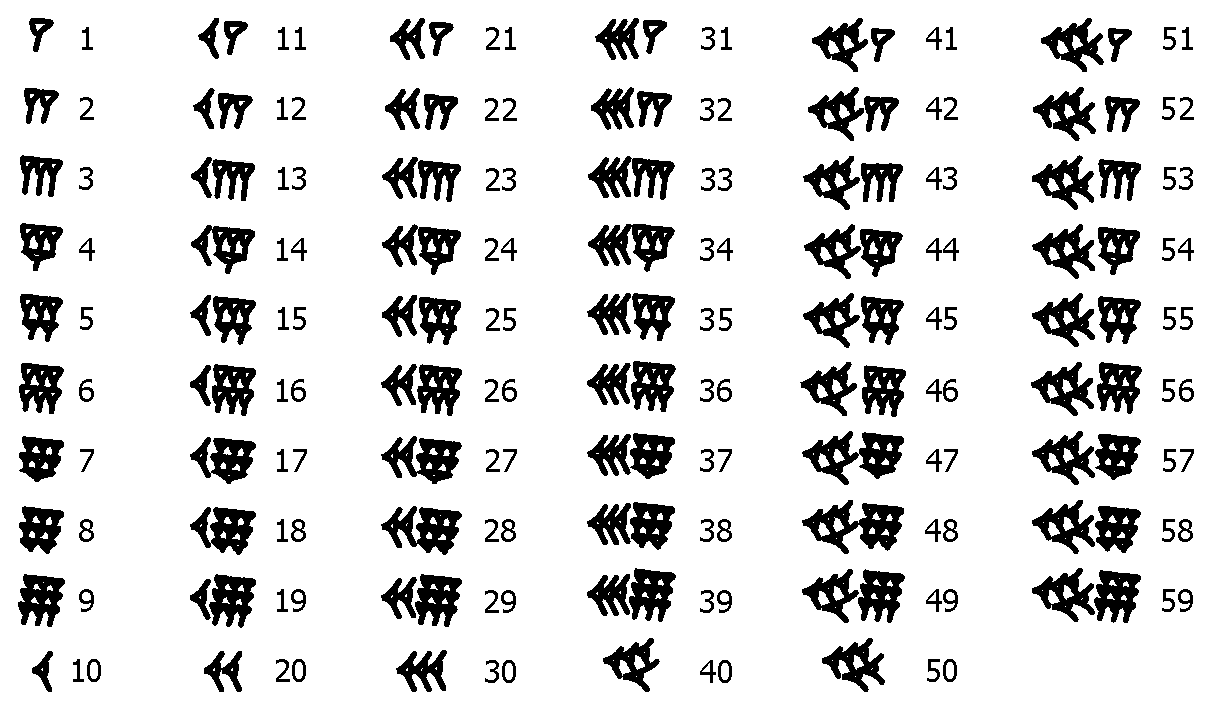
\includegraphics[width=0.9\marginparwidth]{../week1/figures/babylonian.eps}
\caption{The Ancient Babylonians counted using a number system based on the number sixty. They had sixty ``digits'' made using particular marks on cuneiform tablets. Can you imagine having to count with sixty numbers? That makes binary seem positively easy!\attribution{By Josell7, CC BY-SA 4.0, https://commons.wikimedia.org/w/index.php?curid=9862983}}
\label{fig:babylonians}
\end{marginfigure}

\begin{figure}[p]
  \label{fig:just-two} \centering \begin{tikzpicture} \begin{ttboard}[blue
  marbles=8] \TTBit[on]{3}{0} \TTBit[off]{3}{2}

      \TTRamp[right]{4}{1}
      \TTRampRun{4}{1}{\TTRows-2}

      \TTRamp[right]{2}{1}
      \TTInterceptor{2}{3}
    \end{ttboard}
  \end{tikzpicture}
  \caption{Here we have a two-bit machine, but we flipped the top bit so that it starts off pointing right. How many marbles are produced?}
\end{figure}

\subsection{Exploring the Binary Numbers}
\label{sec:binary-numbers}

You're probably familiar with the decimal numbers, which are the numbers we usually count with. The
decimal numbers use ten digits: 0, 1, 2, 3, 4, 5, 6, 7, 8, and 9. To write numbers larger than 9, we
use two digits.\curious{The word \emph{bit} is actually short for \emph{binary digit}.}

For example, to write the number one more than nine, we write ``10''. Then, to write the number one
bigger than that, we have a zero in the one's place, so we have more digits to use. The next digit
after 0 is 1, so the number after 10 is written as ``11''.

It works exactly the same in binary, except we only have two digits: 0 and 1. The binary number 0
means zero and the binary number 1 means one. But how do we write the number two? It's just like
writing the number ten in decimal. Since we don't have another digit, we use two digits. Two can be
written as ``10''.

\didyouknow{There are \emph{infinite} ways of representing numbers. Computer programmers commonly
  use decimal and binary and also two others, known as hexadecimal and octal. We'll cover these
  later.}  This system of using multiple digits to write out numbers for which we do not have enough
digits is called \term{place value}, because the position of the digits in the number representation
is what determines the value.

Let's think about how it works. First, consider some decimal (normal) numbers. We can write out any
two-digit decimal number as the sum of its ten part and its one part:

\[\begin{array}{rcl}
11 &=& 10 + 1. \\
25 &=& 20 + 5. \\
48 &=& 40 + 8.
\end{array}\]

The tens part can further be written as a product of a single digit and the number 10. The numbers
below have their digits colored so you can see where each digit ends up in the sum.

\[\begin{array}{rcl}
\textcolor{blue}{1}\textcolor{red}{1} &=& \textcolor{blue}{1} \times 10 + \textcolor{red}{1}. \\
\textcolor{blue}{2}\textcolor{red}{5} &=& \textcolor{blue}{2} \times 10 + \textcolor{red}{5}. \\
\textcolor{blue}{4}\textcolor{red}{8} &=& \textcolor{blue}{4} \times 10 + \textcolor{red}{8}.
\end{array}\]

What about three digit numbers? Well we can do the same thing, but we use 100 for the third digit, not 10.

\[\begin{array}{rcl}
\textcolor{green}{6}\textcolor{blue}{1}\textcolor{red}{1} &=& \textcolor{green}{6} \times 100 + \textcolor{blue}{1} \times 10 + \textcolor{red}{1}. \\
\textcolor{green}{8}\textcolor{blue}{2}\textcolor{red}{5} &=& \textcolor{green}{8} \times 100 + \textcolor{blue}{2} \times 10 + \textcolor{red}{5}. \\
\textcolor{green}{3}\textcolor{blue}{4}\textcolor{red}{8} &=& \textcolor{green}{3} \times 100 + \textcolor{blue}{4} \times 10 + \textcolor{red}{8}.
\end{array}\]

Of course 100 is just $10 \times 10$:

\[\begin{array}{rcl}
\textcolor{green}{6}\textcolor{blue}{1}\textcolor{red}{1} &=& \textcolor{green}{6} \times 10 \times 10 + \textcolor{blue}{1} \times 10 + \textcolor{red}{1}. \\
\textcolor{green}{8}\textcolor{blue}{2}\textcolor{red}{5} &=& \textcolor{green}{8} \times 10 \times 10 + \textcolor{blue}{2} \times 10 + \textcolor{red}{5}. \\
\textcolor{green}{3}\textcolor{blue}{4}\textcolor{red}{8} &=& \textcolor{green}{3} \times \underbrace{10 \times 10}_{\footnotesize \text{also written }10^2} + \textcolor{blue}{4} \times 10 + \textcolor{red}{8}.
\end{array}\]

We can do something similar for four-digit numbers:
\[\begin{array}{rcl}
\textcolor{orange}{3}\textcolor{green}{6}\textcolor{blue}{4}\textcolor{red}{1} &=& \textcolor{orange}{3} \times \underbrace{10 \times 10 \times 10}_{10^3} + \textcolor{green}{6} \times \underbrace{10 \times 10}_{10^2} + \textcolor{blue}{4} \times 10 + \textcolor{red}{1}. \\
\end{array}\]

As noted above, we can write out repeated multiplications of 10 with itself
as $10^2$, $10^3$, $10^4$.\curious{If $10^2 = 10 \times 10 = 100$ and $10^3 = 10 \times 10 \times 10 = 1000$ what is $10^1$?
  What about $10^0$?}

\[\begin{array}{rcl}
\textcolor{orange}{3}\textcolor{green}{6}\textcolor{blue}{4}\textcolor{red}{1} &=& \textcolor{orange}{3} \times 10^3 + \textcolor{green}{6} \times 10^2 + \textcolor{blue}{4} \times 10 + \textcolor{red}{1}. \\
\end{array}\]

To make the leap to binary numbers, we note that the number 10 is to decimal as the number 2 is to
binary.\curious{The number corresponding to place value number systems is called the
  \term{base}. ``Base 10'' is another way of saying decimal, and ``base 2'' is another name for
  binary.}

Consider the numbers above. We said the binary number ``110'' was decimal number 6. Let's apply the
same rules we did for decimal numbers to ``110''. First, we take each digit. Then we multiply each
digit by the number of twos corresponding to its position.

\curious{It is important to know what base we are dealing with when looking at a particular string
  of digits. In most mathematics, we assume that a number is written in decimal, but if we want to
  be explicit about it, we can write the base of any number in small letters after and below the
  number. For example, the number $110_{10}$ corresponds to the number one hundred and ten. The $10$
  below the $110$ signals that this number is in decimal. Similarly, the number $110_2$ corresponds
  to six.}
\[
\begin{array}{rcl}
  \textcolor{green}{1}\textcolor{blue}{1}\textcolor{red}{0} &=& \textcolor{green}{1} \times 2 \times 2 + \textcolor{blue}{1} \times 2 + \textcolor{red}{0} = 6, \text{or} \\
  \textcolor{green}{1}\textcolor{blue}{1}\textcolor{red}{0} &=& \textcolor{green}{1} \times 2^2 + \textcolor{blue}{1} \times 2 + \textcolor{red}{0} = 6, \text{or} \\
  \underbrace{\textcolor{green}{1}\textcolor{blue}{1}\textcolor{red}{0}}_{\text{in binary}} &=& \textcolor{green}{1} \times 4 + \textcolor{blue}{1} \times 2 + \textcolor{red}{0} = \underbrace{6}_{\text{in decimal}}
\end{array}
\]

This way of expanding numbers is very general and works for all
bases. Its often more convenient to write them out as tables. For
example, consider the decimal number $5837$. We can write it out as:

\hint{These are known as the places:
  the units place\tikzmarknode{week1unitsfrom}, \\
  the tens place\tikzmarknode{week1tensfrom},\\
  the hundreds place\tikzmarknode{week1hundredsfrom}, and \\
  the thousands place\tikzmarknode{week1thousandsfrom}.
}
\begin{center}
  \begin{tabular}{c|c|c|c}
    \hline
    \multicolumn{4}{c}{Place} \\\hline
    \tikzmarknode{week1thousandsto}3 & \tikzmarknode{week1hundredsto}2 & \tikzmarknode{week1tensto}1 & \tikzmarknode{week1unitsto}0 \\\hline
    $10^3$ & $10^2$ & 10 & 1 \\
    $\times$ & $\times$ & $\times$ & $\times$ \\
    5 & 8 & 3 & 7 \\\hline
    5000 + & 800 + & 30 +& 7= \\\hline
    \multicolumn{4}{c}{5837} \\\hline
  \end{tabular}
\end{center}
\tikzbackground{
  \draw[->, gray!20] (week1thousandsfrom.\tikztufteinner) to[bend left] (week1thousandsto.\tikztufteouter);
  \draw[->, gray!20] (week1hundredsfrom.\tikztufteinner) to[bend left] (week1hundredsto.\tikztufteouter);
  \draw[->, gray!20] (week1tensfrom.\tikztufteinner) to[bend left] (week1tensto.\tikztufteouter);
  \draw[->, gray!20] (week1unitsfrom.\tikztufteinner) to[bend left] (week1unitsto.\tikztufteouter);
}

Similarly, we can do the same for a binary number. Consider the \emph{seven-bit} binary number ``1101001'':
\didyouknow{A binary number that can be written in eight or fewer bits is known as a \term{byte}.}

\hint{Similarly, binary has place names corresponding to the numbers
  that are formed by repeatedly multiplying by two:
  the \ordinalnum{64} place\tikzmarknode{week164from},\\
  the \ordinalnum{32} place\tikzmarknode{week132from},\\
  the \ordinalnum{16} place\tikzmarknode{week116from}, \\
  the \ordinalnum{8} place\tikzmarknode{week18from},\\
  the \ordinalnum{4} place\tikzmarknode{week14from},\\
  the twos place, \tikzmarknode{week12from} and \\
  the units place \tikzmarknode{week11from}.}
\begin{center}
  \begin{tabular}{c|c|c|c|c|c|c}
    \hline
    \multicolumn{7}{c}{Place} \\\hline
    \tikzmarknode{week164to}6 & \tikzmarknode{week132to}5 & \tikzmarknode{week116to}4 & \tikzmarknode{week18to}3 & \tikzmarknode{week14to}2 & \tikzmarknode{week12to}1 & \tikzmarknode{week11to}0 \\\hline
    $2^6$ & $2^5$ & $2^4$ & $2^3$ & $2^2$ & 2 & 1 \\
    64 & 32 & 16 & 8 & 4 & 2 & 1 \\
    $\times$ & $\times$ & $\times$ & $\times$ & $\times$ & $\times$ & $\times$ \\
    1 & 1 & 0 & 1 & 0 & 0 & 1 \\\hline
    64 + & 32 + & 0 + & 8 + & 0 + & 0 + & 1 =\\\hline
    \multicolumn{7}{c}{105} \\\hline
  \end{tabular}
\end{center}
\tikzbackground{
  \draw[->, gray!20] (week164from.\tikztufteinner) to[bend right] (week164to.\tikztufteouter);
  \draw[->, gray!20] (week132from.\tikztufteinner) to[bend right] (week132to.\tikztufteouter);
  \draw[->, gray!20] (week116from.\tikztufteinner) to[bend right] (week116to.\tikztufteouter);
  \draw[->, gray!20] (week18from.\tikztufteinner)  to[bend right] (week18to.\tikztufteouter);
  \draw[->, gray!20] (week14from.\tikztufteinner)  to[bend right] (week14to.\tikztufteouter);
  \draw[->, gray!20] (week12from.\tikztufteinner)  to[bend right] (week12to.\tikztufteouter);
  \draw[->, gray!20] (week11from.\tikztufteinner)  to[bend right] (week11to.\tikztufteouter);
}

So the binary number $1101001_2$ corresponds to decimal $105_{10}$.

\begin{TryThisBox}
  Try translating the binary numbers below into the appropriate decimal number using the table and
  the summation methods described above:
  \begin{enumerate}
  \item $0_2$
  \item $10_2$
  \item $101_2$
  \item $111_2$
  \item $10111_2$
  \item $1111101_2$
  \item $10010001_2$
  \item $10000101_2$
  \end{enumerate}
\end{TryThisBox}

\section{From Marbles to Code}

\begin{marginfigure}
  \includegraphics[width=0.8\linewidth]{../week1/figures/alan-turing.jpg}
  \caption{\textbf{Alan Turing} (1912-1954) asked ``What can machines do if they follow
    rules''?. The name \emph{Turing Tumble} comes from Alan Turing. }
\end{marginfigure}

Inside a modern computer, tiny moving things called \emph{electrons} flow through parts that follow
simple rules, just like the pieces on the Turing Tumble board. Some parts remember things, some
parts make decisions, and some parts make sure electrons move in the right direction.

Binary numbers are fundamental to electronic computers because computers represent numbers as
electronic switches that are either on or off, which correspond to binary digits $0_2$ and
$1_2$. The computers you built above are \emph{real} computers, but building very large systems with
them would get complicated. That's why modern computers use electricity.

\begin{BigIdeaBox}
  Whether it uses marbles or electricity, a computer is just a system
  that follows rules.
\end{BigIdeaBox}

Modern computers are built so that you don't need to physically move
pieces to make them do new things. Instead, they can follow many
different rules depending on what you ask them to do.\curious{Every
  computer has a basic set of rules that depends on the physical parts
  inside it. Programming languages like Python are built on top of
  these rules, but we don't need to worry about them yet. This hidden
  layer of rules is sometimes called the \term{computer
    architecture}.}

The process of telling a computer which rules to follow is called \term{programming}. There are many
ways to program a computer. In the Turing Tumble game, we moved pieces physically. On modern
computers, we use something called a \term{programming language}.

One of the simplest programming languages to start with is called
\term{Python}.\aside{Don't worry, this kind of python does not bite! But it is made of bits and \emph{bytes}!}

\subsection{Talking to a Computer}

In this class, we will use the \textbf{Thonny} Python environment.
\aside{Thonny can be downloaded at \href{https://thonny.org}{https://thonny.org}.}

\begin{figure}
  \fixfigure
  \centering
  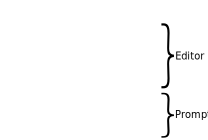
\includegraphics[width=0.9\linewidth]{../week1/figures/thonny-interface.pdf}
  \caption{The Thonny interface. The interface is split into two
    parts: (1) the editor and (2) the prompt.}
  \label{fig:thonny-interface}
\end{figure}

We can talk to Python by entering ``rules'' into the prompt (see
\prettyref{fig:thonny-interface}) and immediately seeing what
happens. This is like dropping a marble into the machines we built
earlier and watching what happens.  \didyouknow{Long before modern
  computers, scholars attempted to study \emph{human} language through
  using rules. One such scholar was the Indian grammarian
  P\={a}\d{n}ini. Around 500 BC, he described the Sanskrit language
  using a precise set of rules that could combine to generate all
  valid sentences in that language!}

In Turing Tumble, our rules were made of plastic pieces. In Python, we
use special words and symbols to write rules.

Let's type our first rule! The simplest rules (also known as \term{expressions})
are the ones that stand for numbers. We can enter these rules by
typing in a number and pressing the Enter or Return key.

Try entering these into the Thonny prompt, and see what
happens.\hint{Type each line one at a time and observe what happens.}

\begin{replbox}
1<ENTER>
54<ENTER>
0<ENTER>
\end{replbox}
\hint{The response from the computer to each of these should be
  numbers. If it's not, you may have typed it in incorrectl. Try it
  again. If that still doesn't work, see \prettyref{sec:errors}}

The rule for numbers is that when you enter them in, you get the same
number out!

\begin{BigIdeaBox}
  Just like the ball thrown up in the air, and just like the
  machines we built, every time you run these rules, the answer is the
  same!
\end{BigIdeaBox}

Python understands many different kinds of numbers. By default, Python uses decimal numbers, as we'd
expect, but we can also use binary numbers. We write binary numbers by putting \code{0b} in front of
the number. Python will respond back in decimal.

\begin{replbox}
0b1<ENTER>
0b101<ENTER>
0b1101<ENTER>
\end{replbox}

We can also ask Python to write a decimal number in binary using \code{bin()}.

\hint{From now on, all the rules we see will be
    \emph{colored}. You don't need to enter the colors in. The colors
    only serve to make the rules easier to read. This is called
    \term{syntax highlighting}.}
\begin{replbox}
bin(10)<ENTER>
bin(1)<ENTER>
bin(2)<ENTER>
bin(3391249)<ENTER>
\end{replbox}

Let's try something more complicated. Before trying the following
rules, think about what is going to happen. A good programmer tries to
predict the output before they use the rule.  \curious{When you type
  something into Python and press Enter, the computer always produces
  the same result for the same input. This idea is called
  \term{determinism}.}

\begin{replbox}
1 + 1<ENTER>
5 - 3<ENTER>
4 * 3<ENTER>
\end{replbox}

\subsection{How Computers Follow Rules}

The symbols we used above connected two number rules together. When we
pressed enter, we got a new number, which is itself a kind of
rule. The way this number was generated depended on the exact symbol
we used. You're probably familiar with the \code{+} symbol, which
means addition. Can you guess what the \code{*} symbol stands for?
If you guessed multiplication, you're right. \hint{You're probably
  familiar with the symbol $\times$ for multiplication, but that
  symbol is hard to type! Most programming languages use \code{*} to
  denote multiplication.}

Since Python lets us combine rules however we want, we can combine
rules involving both multiplication and addition. Before trying the
exercises below, try to guess what the answer is and write down why.

\begin{replbox}
4 + 2 * 3<ENTER>
2 * 3 + 4<ENTER>
\end{replbox}

You may be surprised that the these rules both produced the same number.

In many programming languages, including Python, symbols like
\code{+} and \code{*} have rules to determine which one goes
first. In this case, multiplication always goes first.\curious{\term{Operator precedence} rules determine which written rules get done first.}

Sometimes it can help to \emph{draw} the expressions to figure out
exactly what is going on as in \prettyref{fig:parenrules}.

% TODO figure that shows how to make these into trees

What if we want to make additions occur first? We can always use
parentheses (that is \code{(} and \code{)}) around rules we want to
execute first.

\begin{replbox}
2 * 3 + 4<ENTER>
2 * (3 + 4)<ENTER>
\end{replbox}\hint{Remember it's always a good idea to \emph{predict} what is going to happen \emph{before} hitting the Enter key.}

In this case, the parentheses force the \code{3 + 4} rule to execute
first. \prettyref{fig:parenrules} shows how the diagram for this rule
looks different than the diagram for the \code{2 * 3 + 4} rule.

\begin{figure}
  \fixfigure
  \begin{minipage}{0.45\linewidth}
    \centering
    \begin{forest}
      [{*}
        [2]
        [{+} [3] [4]]]
    \end{forest}
  \end{minipage}
  \begin{minipage}{0.45\linewidth}
    \centering
    \begin{forest}
      [{+}
        [{*}
          [2]
          [3]]
        [4]]
    \end{forest}
  \end{minipage}
  \caption{The rule \code{2 * (3 + 4)} is drawn differently than the rule \code{2 * 3 + 4}.}
  \label{fig:parenrules}
\end{figure}

\begin{BigIdeaBox}
  When rules combine, there are rules to determine which rule go
  first. No matter which rules we are talking about, they always
  behave in \emph{exactly} the same way.
\end{BigIdeaBox}

There's one more thing to think about. What if we put parentheses around the
multiplication?\hint{It's always good to remember that computers don't think about \emph{why} they
  do something. They only know \emph{what} to do!}

\begin{replbox}
2 * 3 + 4<ENTER>
(2 * 3) + 4<ENTER>
\end{replbox}
\hint{At this point, you probably know you need to \emph{predict} what is going to happen before proceeding!}

In this case, it again helps to draw it out. As you can see both of
these rules can be represented by the same diagram (see
\prettyref{fig:paren-mult}). Since the diagrams match, the rules mean
the same thing even though they're typed out differently.
\curious{Electronic computers are structured as layers of rules. A
  really hard-working computer programmer made rules that told Python
  what to do to understand the rules you type in to the
  computer. Those rules were typed out in another language called
  C. Another program called a \term{compiler} took those rules and
  generated yet more sets of rules. Its rules all the way down!}

\begin{BigIdeaBox}
  The same rule can be typed out many different ways! We can apply the
  rules for diagramming rules to see if they mean the same
  thing.
\end{BigIdeaBox}

\begin{figure}
  \fixfigure
  \centering
  \begin{forest}
  [{+}
   [{*} [2] [3]]
   [4]]
  \end{forest}
  \caption{The rule \code{2 * 3 + 4} and \code{(2 * 3) + 4} are
    represented by the same diagram even though they are typed out
    differently.}
  \label{fig:paren-mult}
\end{figure}

\subsection{Rules with Words}

So far, all our rules have involved numbers, but computers can handle
more than that. Computers can also follow rules about
\emph{words}.\didyouknow{Python actually has \emph{two} kinds of
  numbers, but we will have to come back to that later.}

\begin{replbox}
"hello"<ENTER>
"my name is Bob"<ENTER>
\end{replbox}
\hint{Words must be surrounded by \code{"}s or you will get an
  error. Make sure you type everything in exactly as written.}

You'll notice that Python responds back with the word (or phrase) you
put in. \didyouknow{Programmers use the term \term{strings} to refer to
  rules representing words in programs.}

Now try this, but remember to \emph{predict} what is going to happen
before typing it in.\huh{But I thought
  \code{+} added numbers together. How come I can use it with
  words?}{Some symbols like \code{+} can do different things depending
  on whether it is used with words or numbers. Different programming
  languages have different rules regarding which combinations of
  simbols, words, and numbers are allowed and what exactly they
  mean. The technical term for this is \term{operator overloading}. A
  useful list of these rules in Python is given in
  \prettyref{tab:operator-rules-1}}

\begin{replbox}
"hello " + "world"<ENTER>
\end{replbox}

Did it do what you expected? If you typed it in correctly, Python
should have responded with \code{"hello world"}.

We've now seen a rule involving words! When you use \code{+} on two
words, you get those two words put together. What else can we do with words?

\begin{replbox}
"ho" * 3<ENTER>
\end{replbox}

You should see the response \code{"hohoho"}, which is just \code{"ho"}
repeated three times. \hint{Python did not suddenly decide to be
  festive. The word returned is the result of Python applying its set
  of rules \emph{exactly} to what you wrote.}

\begin{TryThisBox}
Can you multiply a word by another word? What would this mean? Think
about it, before we find out the answer in the next section.
\end{TryThisBox}

\begin{marginfigure}
  \centering
  \includegraphics[width=0.9\marginparwidth]{../week1/figures/game-of-life.png}
  \caption{The Game of Life by John Conway is a system that follows simple rules that can create complex behavior. Above is an example of expressing a rule in the Game of Life. See the Deep Dive Box on page \pageref{box:gameoflife} for more information.\attribution{Hyperdeath, CC BY-SA 3.0 <https://creativecommons.org/licenses/by-sa/3.0>, via Wikimedia Commons}}
\end{marginfigure}

\subsection{Some Rules Don't Make Sense}
\label{sec:errors}

Remember that when we type rules, Python applies more rules to make
sense of what we typed. We can visualize these rules by drawing
diagrams. But sometimes, we write something that Python's rules cannot
figure out. Although we can type them using the keyboard they don't
make sense to Python. This would be like trying to place two Turing
Tumble pieces on one peg when building a machine -- it just doesn't
make sense. We call these issues \term{syntax errors}.

\begin{replbox}
2 + 5 +<ENTER>
* 4<ENTER>
\end{replbox}

Other times we type rules that Python understand, but when it tries to
process them, it gets confused. This is like placing a much larger
marble into the Turing Tumble game -- although our placement of pieces
makes sense, we cannot make the pieces move with the wrong type of
marble. This is called a \term{runtime error}. You may have also heard
it called a \term{bug}. \didyouknow{The first computer bugs were
  caused by actual bugs that got stuck in hot electronic parts used in
  the earliest electric computers. Yuck!}

Both of these issues are kinds of \term{errors}.

\begin{BigIdeaBox}
  Python always applies the same rules to understand and process our
  rules, but sometimes what we put in doesn't make sense.
\end{BigIdeaBox}

In Python, errors are reported back to us as they occur, and Python
tries to give us information that can help us correct the error.
\hint{Although it may seem scary, there is nothing ``wrong'' with an
  error. It's just the computer applying rules and telling you
  something doesn't make sense.}

Although Python will provide some information that can be useful to
fix our program, Python is itself a collection of rules, and its rules
may not fully understand what we are trying to do based on what we
input. This is where the job of a programmer becomes important.

See \prettyref{tab:python-errors} for examples of some errors we
might encounter as we continue with our learning. You don't need to
memorize these, but it may be useful to refer back.

\begin{table}
  \fixfigure

\begin{tabularx}{\linewidth}{lp{0.6\linewidth}}
\toprule
\code{NameError} & A name of a rule was mistyped (i.e., you typed \code{length} instead of \code{len}). \\
\code{TypeError} & You used a number where a word was expected or vice versa (i.e., \code{'hello'/2}). \\
\code{ZeroDivisionError} & You tried to divide a number by zero. Uh-oh! \\
\code{SyntaxError} & Python couldn't make sense of what you typed because it didn't follow Python's rules (i.e., you typed \code{2 + 5 *} and python doesn't know what to multiply 5 by). \\
\code{OverflowError} & Some kinds of calculations on numbers can result in very large numbers that don't fit into the computer. \\\bottomrule
\end{tabularx}

\caption{As we continue in our learning, we will most likely encounter more errors. Errors are a
  \emph{normal} part of programming. They do not mean anything is broken! It just means there's been
  a misunderstanding between what you thought was going to happen and what actually happened when
  the computer followed through exactly with the rules you set out for it. Instead of being
  discouraged, think of every error as an opportunity learn \emph{more}!}
\label{tab:python-errors}
\end{table}

\section{Conclusion}

Computers follow rules exactly. When we program a computer, we make
new rules for the computer to follow. In Python, simple rules can
involve numbers and words. Sometimes, the rules we write don't make
sense. This is called an error, but is still the result of the
computer following a set of rules.

We haven't learned how to program \emph{yet}, but we have started
toying with the idea of turning ideas into instructions. When we do
this, the small details really matter. Missing pieces can cause
confusion. Unclear instructions lead to unexpected results. When
things go wrong, it's not because the computer was wrong, but because
it followed the instructions exactly as written.

This is computer's greatest strength. They never guess or fill in
missing steps. They just do exactly what you tell it! Computer science
is not about memorizing commands or tying a lot. It's about learning
how to say things clearly enough that a process -- whether a table
game, machine, or a person -- can follow your ideas without confusion.

In the next chapter we'll start to think deeper about how to precisely
describe to the computer the things we want to make.

\begin{DeepDiveBox}
  \boxtitle{Simple Rules, Surprising Worlds: The Game of Life}
  \label{box:gameoflife}

  One of the most famous rule-based systems ever created is called the \emph{Game of Life}, invented
  by mathematician John Conway.

  Despite the name it isn't really a game -- it's a world that follows rules.

  Imagine a giant sheet of graph paper. Each square can either be \emph{alive} or
  \emph{dead}. That's it. No colors, no thinking, nothing. Just alive or dead.
  \margmark{play-life}{\curiousboxtext You can play the game of life by going to \href{https://playgameoflife.com}{https://playgameoflife.com}.\\
    \begin{center}
      \qrcode{https://playgameoflife.com}
  \end{center}}

  The game proceeds in turns. At each turn, each square looks at its eight neighbors and follows
  these simple rules (all squares update at the same time):
  \begin{enumerate}
  \item If a square is \emph{alive} and has fewer than two live neighbors, it gets lonely and dies.
  \item If a square is \emph{alive} and has two or three live neighbors, it stays alive.
  \item If a square is \emph{alive} and has more than three live neighbors, it suffocates and dies.
  \item If a square is \emph{dead} and has exactly three live neighbors, it comes to life.
  \end{enumerate}
  \margmark{gameofliferules}{
      Each turn, a cell looks at its neighbors and decides to either come to life, stay alive, or die. \\
      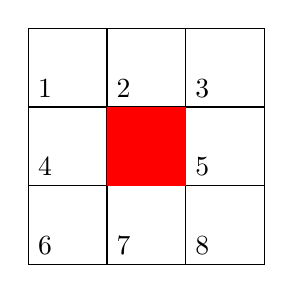
\begin{tikzpicture}
        \foreach \x in {0,1,2} {
          \foreach \y in {0,1,2} {
            \draw (\x,\y) rectangle ++(1,1);
          }
        }
        \fill[red] (1,1) rectangle ++(1,1);
        \node [anchor=south west] at (0, 2) {1}; % top-left
        \node [anchor=south west] at (1, 2) {2}; % top-middle
        \node [anchor=south west] at (2, 2) {3}; % top-right
        \node [anchor=south west] at (0, 1) {4}; % middle-left
        \node [anchor=south west] at (2, 1) {5}; % middle-right
        \node [anchor=south west] at (0, 0){6}; % bottom-left
        \node [anchor=south west] at (1, 0) {7}; % bottom-middle
        \node [anchor=south west] at (2, 0) {8}; % bottom-right
      \end{tikzpicture}
    }

  \textbf{\sffamily \large What Happens?}

  Surprisingly, this system is a \emph{full} computer and can compute \emph{anything}. You can build
  patterns that do all sorts of things. Some patterns move across the board. Some repeat
  forever. Some patterns build other patterns.

  All of this comes from just four simple rules!

  The Game of Life shows something very important: \textbf{Simple rules can create behavior that
    looks alive, planned, or intelligent -- even when nothing is thinking}. This is the same idea
  behind the electronic computers that we use every day.
\end{DeepDiveBox}

\Exercises

\curious{Exercises are fun things you can try at home}

\begin{exercises}
\item Construct Turing Tumble boards that do the following:
  \begin{enumerate}
  \item Construct an alterating sequence of marbles \ttpieces{rbrbrbrb}\ldots?
    \answer{}
  \item Returns a sequence of alternating marbles one red, two blue like \ttpieces{rbbrbbrbb}\ldots?
  \item In class, we built boards to count out a number of marbles. We used sequences of bits to do
    this. These sequences are known as \emph{registers}. Can you build a board that takes a binary
    number in a register and \emph{adds one} to that binary number?
  \item Can you extend the board you made above to contain two separate registers and have the board
    add the two binary numbers together? Try one-bit and two-bit registers. What limits do you run
    up against as you try to increase the number of bits?
  \end{enumerate}

\item Figure out the rule that the following Turing Tumble boards follow when a blue ball is released first:
  \begin{tasks}(2)
  \task \answer{It produces one blue marble and then all the red marbles}
    \begin{tikzpicture}[baseline=(ttboardtop.base)]
    \begin{ttboard}[margin, blue marbles=5, red marbles=5, blue marbles released=1, output={\Large ?}]
      \TTRamp[right]{3}{0}
      \TTRamp[left]{7}{0}
      \TTRamp[right]{4}{1}
      \TTRamp[left]{6}{1}
      \TTRamp[right]{5}{2}
      \TTRamp[right]{6}{3}
      \TTRamp[right]{7}{4}
      \TTRampRun{8}{5}{\TTRows - 2}
    \end{ttboard}
    \end{tikzpicture}

  \task \answer{It produces an alternating run of marbles \ttpieces{brbrbrb}\ldots}
    \begin{tikzpicture}[baseline=(ttboardtop.base)]
      \begin{ttboard}[margin, blue marbles=5, red marbles =5, blue marbles released=1, output={\Large  ?}]
        \TTRamp[right]{3}{0}
        \TTRamp[left]{7}{0}
        \TTRamp[right]{4}{1}
        \TTRamp[left]{6}{1}
        \TTCrossover{5}{2}
        \TTRampRun{3}{3}{\TTRows - 2}
        \TTRampRun{6}{3}{\TTRows - 2}
      \end{ttboard}
    \end{tikzpicture}

  \task \answer{It produces an alternating run of marbles \ttpieces{brbrbrb}\ldots}
    \begin{tikzpicture}[baseline=(ttboardtop.base)]
      \begin{ttboard}[margin, blue marbles=5, red marbles =5, blue marbles released=1, output={\Large ?}]
        \TTRamp[right]{3}{0}
        \TTRamp[left]{7}{0}
        \TTRamp[right]{4}{1}
        \TTRamp[left]{6}{1}
        \TTBit{5}{2}
        \TTRamp[left]{4}{3}
        \TTRamp[right]{6}{3}
        \TTRampRun{3}{4}{\TTRows - 2}
        \TTRampRun{6}{4}{\TTRows - 2}
      \end{ttboard}
    \end{tikzpicture}

  \task \answer{It produces four blue marbles and then only red marbles.}
    \begin{tikzpicture}[baseline=(ttboardtop.base)]
      \begin{ttboard}[margin, blue marbles=5, red marbles =5, blue marbles released=1, output={\Large ?}]
        \TTBit[on]{3}{0}
        \TTBit[on]{3}{2}
        \TTRampRun{1}{1}{\TTRows - 2}
        \TTRamp[left]{4}{1}
        \TTRamp[right]{4}{3}
        \TTRamp[right]{5}{4}
        \TTRamp[right]{6}{5}
        \TTRamp[left]{7}{6}
        \TTRamp[left]{7}{0}
        \TTRamp[right]{6}{1}
        \TTRamp[right]{7}{2}
        \TTRamp[left]{8}{3}
        \TTRamp[left]{7}{4}
        \TTRamp[left]{6}{5}
        \TTBit[off,gear]{5}{6}
        \TTGear{4}{6}
        \TTBit[off,gear]{4}{7}
        \TTRamp[left]{6}{7}
        \TTRamp[right]{5}{8}
        \TTRamp[right]{6}{9}
      \end{ttboard}
    \end{tikzpicture}
  \end{tasks}
\item Predict the answer to the following Python rules:
  \begin{enumerate}
  \item \code{1 \enterkey}\answer{1}
  \item \code{-1 \enterkey}\answer{-1}
  \item \code{3 + 2 \enterkey}\answer{5}
  \item \code{3 * 9 + 6 \enterkey}\answer{35}
  \item \code{6 * 3 * 2 \enterkey}\answer{36}
  \item \code{6 + 3 + 2 \enterkey}\answer{11}
  \item \code{6 * 4 - 8 * 2 \enterkey}\answer{8}
  \item \code{6 * 4 // 2 \enterkey}\hint{Remember that \code{//} means division in Python}\answer{12}
  \end{enumerate}

\item Try the following rules.
  \begin{enumerate}
  \item \code{len(``a'')}
  \item \code{len(``ab'')}
  \item \code{len(``abc'')}
  \item \code{len("")}
  \end{enumerate}
  What does the \code{len} rule do?
  \answer{It calculates how many letters are in the word.}
\end{exercises}

\begin{table*}
  \begin{tabularx}{\linewidth}{llL}
      \toprule
      \headercol{Symbol} & & \headercol{Meaning} \\\midrule
      {\ttfamily *, //, \%} & \code{number * number} & Multiply two numbers together \\
      & \code{number // number} & Divide two numbers \\
      & \code{number \% number} & The remainder when dividing the numbers \\
      & \code{word * number} & Repeat the word this many times \\\hline
      {\ttfamily +, -} & \code{number + number} & Add two numbers together \\
      & \code{number - number} & Subtract the second number from the first \\
      & \code{word + word} & Combine the two words together \\
      \code{len} & \code{len(word)} & Get the number of letters and digits in the word \\
      \code{bin} & \code{bin(number)} & Get the binary number corresponding to the number \\\bottomrule
  \end{tabularx}
  \caption{This is a list of symbols you can use to combine rules in
    Python. Symbols that appear first are executed first, unless you
    use parentheses to force some rules to ge first. The behavior of
    symbols can depend on whether it's used with numbers or words. All
    these variants are given here}
  \label{tab:operator-rules-1}
\end{table*}
